\documentclass[border=4pt]{standalone}
\usepackage{amsmath,amssymb,amsfonts}
\usepackage{xcolor,colortbl,array,booktabs,multirow}
\usepackage{tikz}
\usepackage{pgfplots}
\pgfplotsset{compat=1.16}
\usetikzlibrary{arrows, automata, backgrounds, calendar, chains, decorations,
    matrix, mindmap, patterns, petri, positioning, shadows, shapes.geometric,
    trees, shapes, decorations.pathreplacing, calc, tikzmark, arrows.meta,
    intersections, fit, graphs, quotes, angles, decorations.markings}
\newcommand{\st}{\text{ s.t. }}
\newcommand{\x}{\mathbf{x}}
\renewcommand{\b}{\mathbf{b}}
\renewcommand{\c}{\mathbf{c}}
\newcommand{\A}{\mathbf{A}}
\newcommand{\y}{\mathbf{y}}
\newcommand{\z}{\mathbf{z}}
\newcommand{\R}{\mathbb{R}}
\newcommand{\RR}{\mathbb{R}}
\newcommand{\Z}{\mathbb{Z}}
\newcommand{\ZZ}{\mathbb{Z}}
\newcommand{\npcomplete}{NP-complete}
\providecommand{\true}{\text{TRUE}}
\providecommand{\false}{\text{FALSE}}
\tikzset{vertex/.style={circle,fill=black!25,minimum size=20pt,inner sep=0pt},
    edge/.style={draw,thick,-},weight/.style={font=\small},
    selected vertex/.style={vertex, fill=red!24},
    selected edge/.style={draw,line width=2pt,-,red!50},
    ignored edge/.style={draw,line width=2pt,-,black!20}}
\newcommand{\vect}{\vec}
\providecommand{\ds}{\displaystyle}
\providecommand{\longvect}{\overrightarrow}
\usepackage[normalem]{ulem}
\definecolor{ocre}{RGB}{243,102,25}
\providecommand{\leftB}{\left[}
\providecommand{\rightB}{\right]}
\tikzset{directed/.style={postaction={decorate,decoration={markings,mark=at position .65 with {\arrow{>}}}}},
    directed1/.style={postaction={decorate,decoration={markings,mark=at position .65 with {\arrow{>}}}}}}
\begin{document}
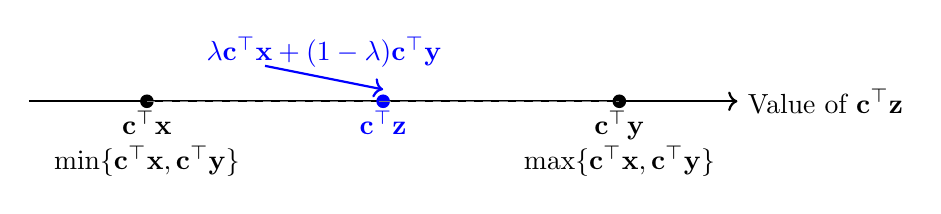
\begin{tikzpicture}[scale=1.5]
    % Draw the 1D line
    \draw[thick, ->] (0, 0) -- (6, 0) node[right] {Value of $\mathbf{c}^\top \mathbf{z}$};

    % Points for c^T x, c^T y, and c^T z
    \filldraw[black] (1, 0) circle (1.5pt) node[below] {$\mathbf{c}^\top \mathbf{x}$};
    \filldraw[black] (5, 0) circle (1.5pt) node[below] {$\mathbf{c}^\top \mathbf{y}$};
    
    % Point for c^T z (somewhere in between)
    \filldraw[blue] (3, 0) circle (1.5pt) node[below] {$\mathbf{c}^\top \mathbf{z}$};

    % Annotate convex combination
    \draw[dashed, gray] (1, 0) -- (3, 0);
    \draw[dashed, gray] (3, 0) -- (5, 0);

    % Add min and max bounds
    \node[below] at (1, -0.3) {$\min\{\mathbf{c}^\top \mathbf{x}, \mathbf{c}^\top \mathbf{y}\}$};
    \node[below] at (5, -0.3) {$\max\{\mathbf{c}^\top \mathbf{x}, \mathbf{c}^\top \mathbf{y}\}$};

    % Add explanation arrow for convex combination
    \draw[->, thick, blue] (2, 0.3) -- (3, 0.1) node[midway, above] {$\lambda \mathbf{c}^\top \mathbf{x} + (1-\lambda) \mathbf{c}^\top \mathbf{y}$};

\end{tikzpicture}
\end{document}
